\documentclass[14pt]{beamer}

\usepackage[ngerman]{babel}
\usepackage[utf8]{inputenc}
\usepackage{graphicx,hyperref,ru,url}
\usepackage{amsmath}
\usepackage{amssymb}
\usepackage{color}
\usepackage[export]{adjustbox}
\setbeamerfont{frametitle}{size=\normalsize}

\title[AlgoKarto]{Algokarto Projekt}
%\subtitle{}

\author[Maximilian Vogel, Florian Becker]{Maximilian Vogel, Florian Becker}
%\institute[]{}
\date[9.Juli 2015]{9.Juli 2015}


%%%%%%%%%%%%%%
%%%%%%%%%%%%%%
\begin{document}

\begin{frame}
\large
  \titlepage
\end{frame}

\begin{frame}{de Berg Algorithmus}
  \begin{itemize}
        \item Tangentensplitter berechnen
        \item Punkte verteilen
        \item konsistente Shortcuts filtern
  \end{itemize}

  
  \begin{block}{Laufzeit}
     $O(N(N+M)log(N))$
  \end{block}
 
\end{frame}

\begin{frame}{de Berg Algorithmus - Tangentensplitter}
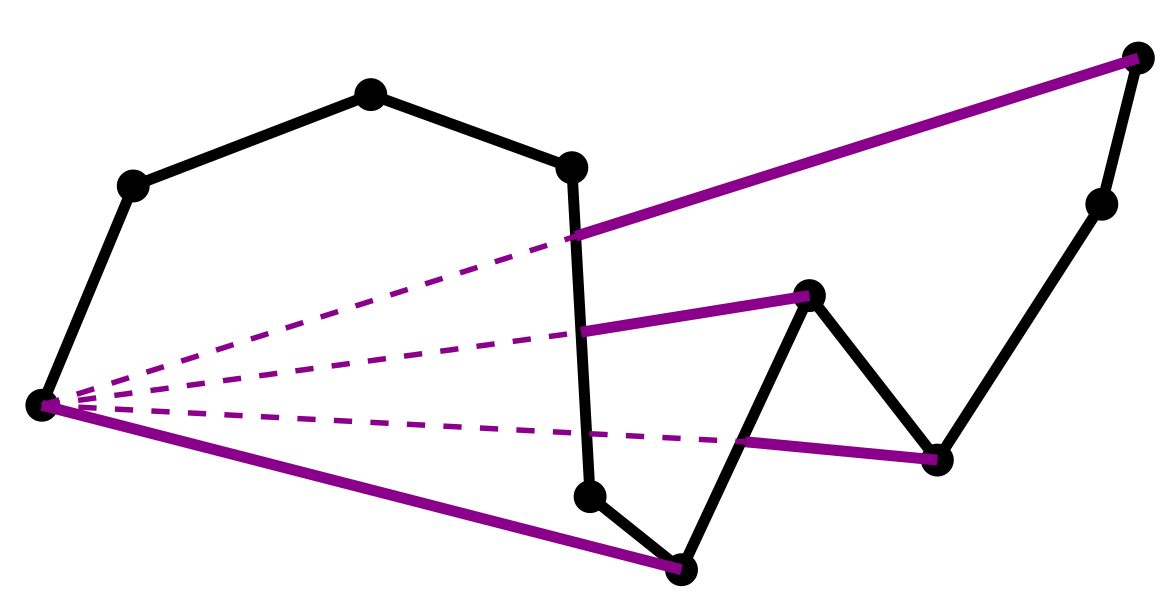
\includegraphics[width=1.0\textwidth]{img/tangentsplitter.png}
\end{frame}

\begin{frame}{de Berg Algorithmus - Punkte verteilen}
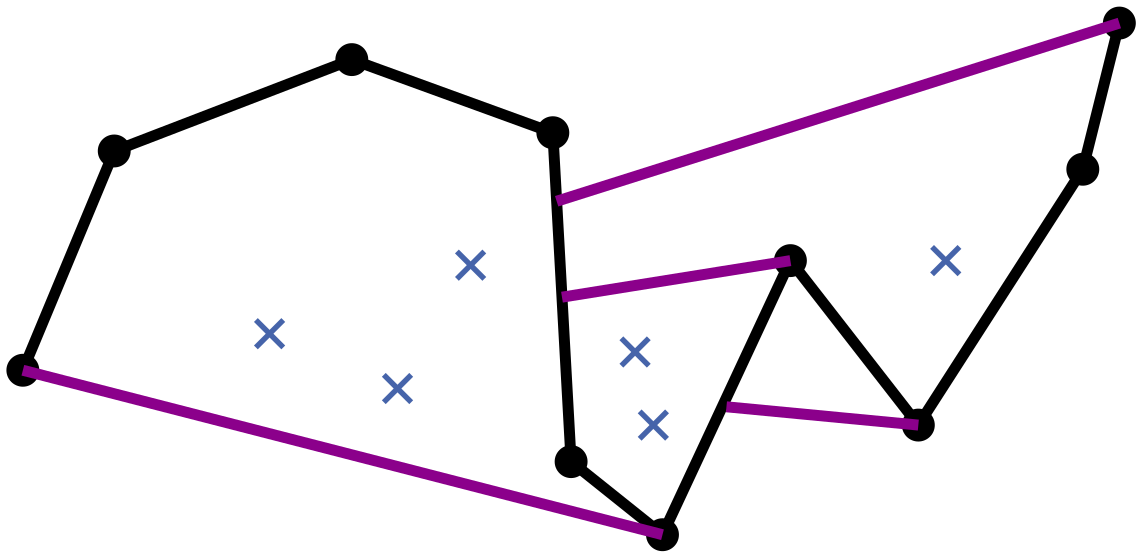
\includegraphics[width=1.0\textwidth]{img/distributepoints.png}
\end{frame}

\begin{frame}{de Berg Algorithmus - konsistente Shortcuts filtern}
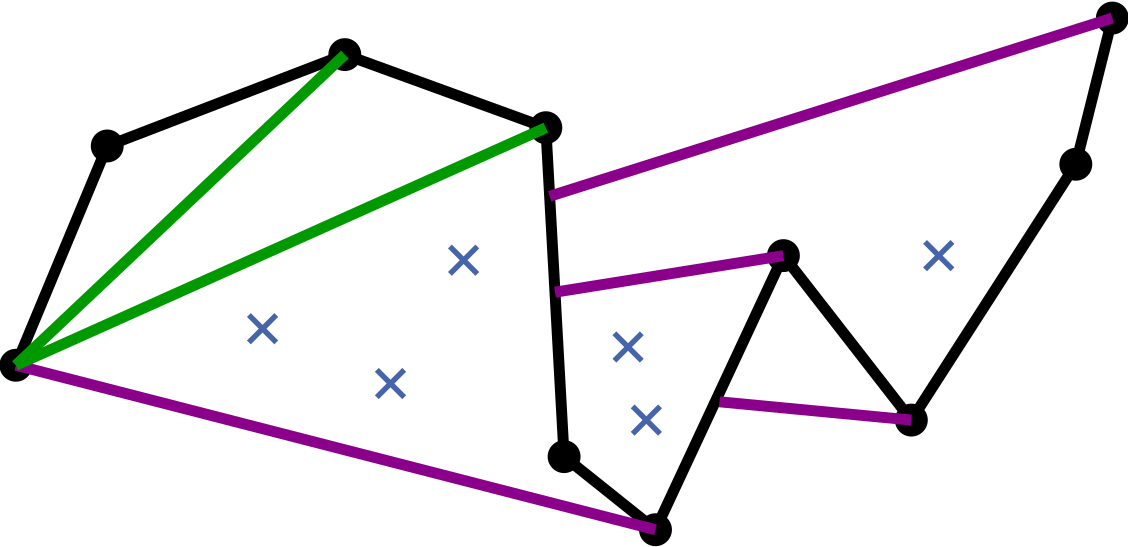
\includegraphics[width=1.0\textwidth]{img/discard_accept.png}
\end{frame}

\begin{frame}{de Berg Algorithmus}
  \begin{itemize}
  	\item \textbf{Problem:} Algorithmus nur auf x-monotone Polygonzüge definiert
	\item \textbf{Lösungsansätze:}
		\begin{itemize}
			\item Koordinatentransformation und Auftrennen
			\item längsten Teilpolygonzug für jeden Punkt
		\end{itemize}
  \end{itemize}
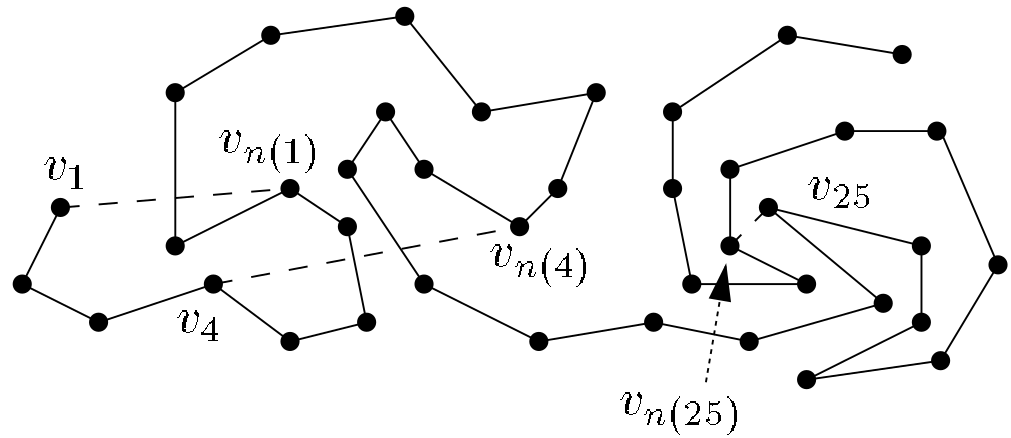
\includegraphics[width=1.0\textwidth]{img/determineSubchain.png}  
\end{frame}

\begin{frame}{Implementierung}
\begin{itemize}
	\item Python, unoptimiert
	\item ''Prosa''-pseudocode kann ausarten: \emph{''search in $T$ to find the leftmost edge $\overline{v_kv_{k+1}}$ to the right of $p$ and on the
sweep-line''}
\end{itemize}

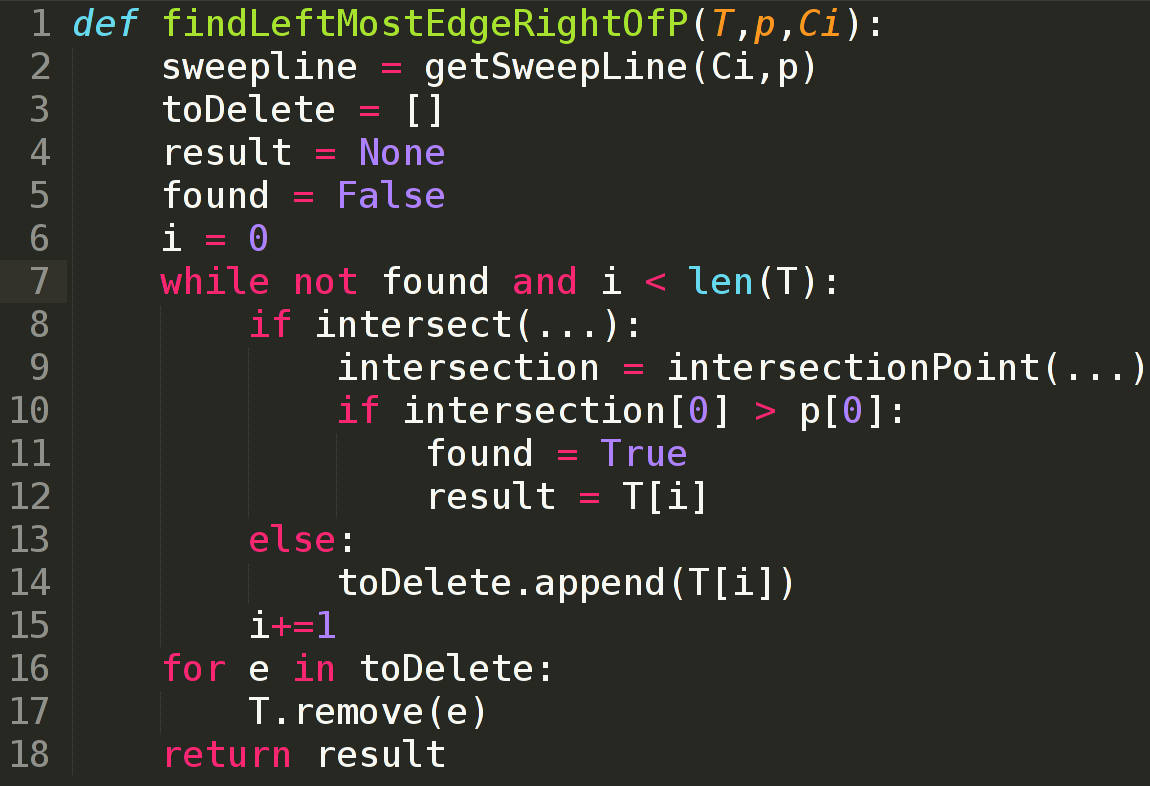
\includegraphics[width=.8\textwidth,center]{img/implvspseudo.png}
\end{frame}

\begin{frame}{Ergebnisse}
\begin{itemize}
	\item Testdatensatz 1: $965 \rightarrow 494$
	\item Testdatensatz 2: $1518 \rightarrow 710$
	\item BaWü: $451145 \rightarrow 109580$
\end{itemize}
\end{frame}

\begin{frame}{Ergebnisse}
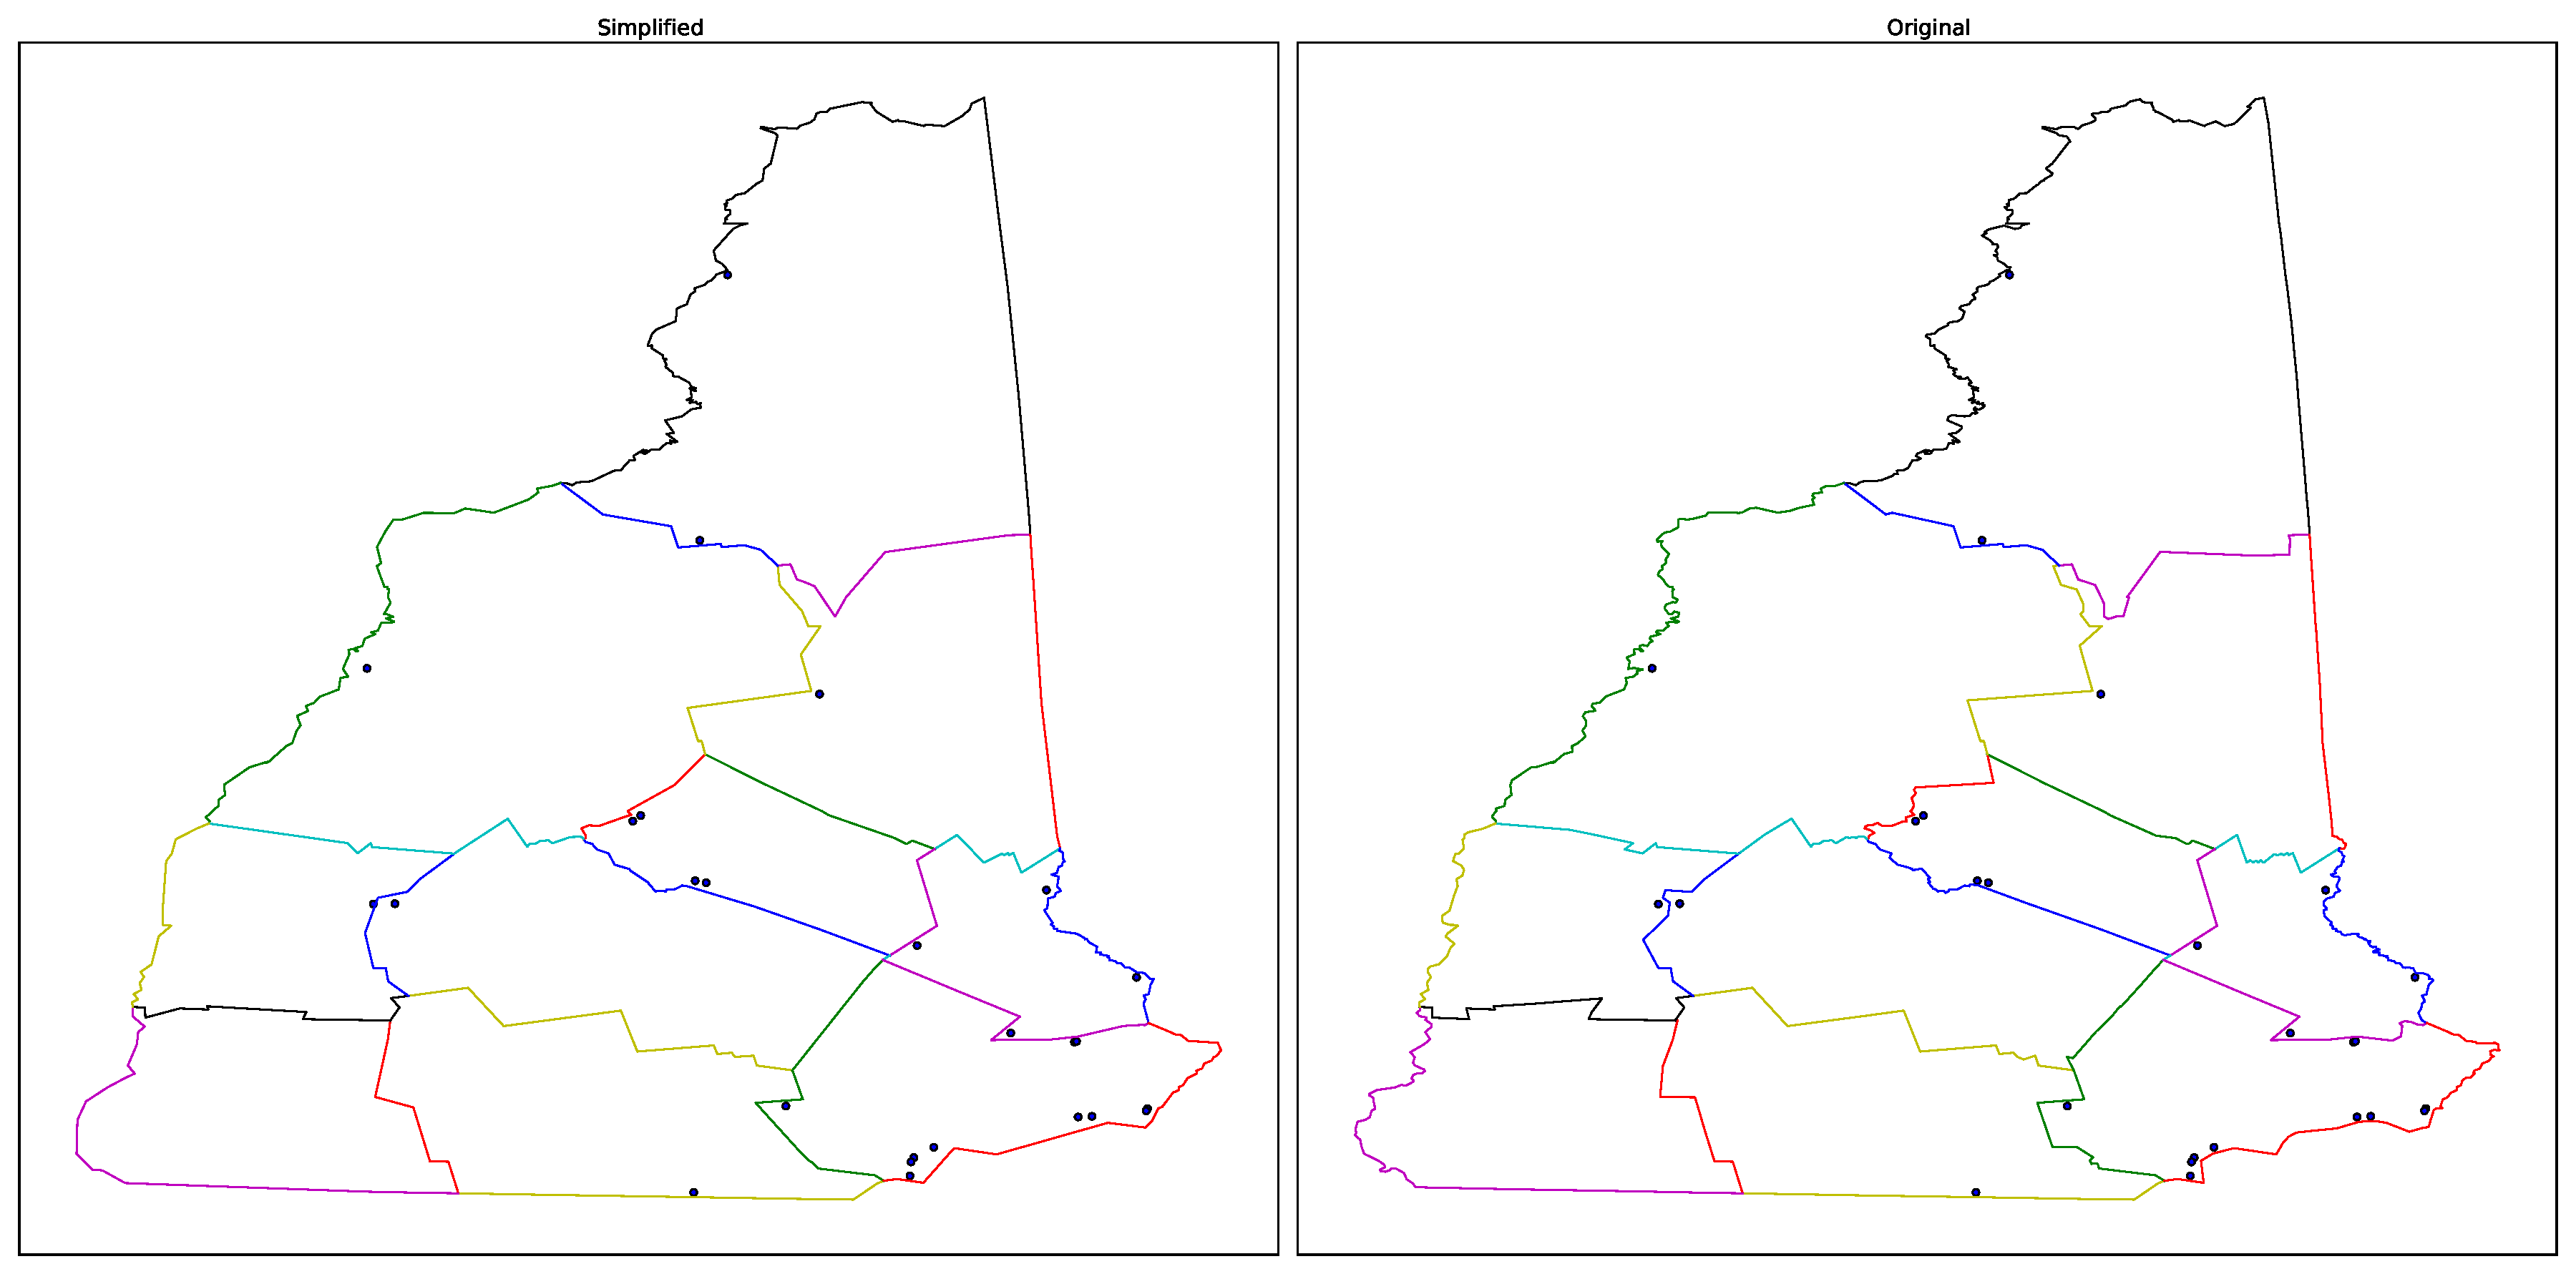
\includegraphics[width=1.25\textwidth,center]{img/result_dataset1.pdf}
\end{frame}

\begin{frame}{Ergebnisse}
\includegraphics[width=1.25\textwidth,center]{img/result_dataset2.pdf}
\end{frame}


\begin{frame}{Fazit}
  \begin{itemize}
	\item Preprocessing der einschränkenden Punktemenge
	\item Algorithmus von beiden Seiten starten (?)
	\item \dots
\end{itemize}
\end{frame}

\end{document}
